\documentclass[10pt]{beamer}
\usetheme{jambro}

\title[]{Pensamento Econômico Contemporâneo - Ciclos Reais de Negócios}
\author[]{Paulo Victor da Fonseca}
\date{}

\hypersetup{
    colorlinks = true,
    urlcolor = teal,
    linkcolor = teal    
}
\usepackage[portuguese]{babel}
\usepackage{subfig}
\usepackage{emoji}

\begin{document}

\begin{frame}[plain]
    \titlepage{
        \begin{center}
            \begin{minipage}{0.8\textwidth}
                \centering
            \end{minipage}
        \end{center}}
\end{frame}

\begin{frame}{Sumário}
    \tableofcontents
\end{frame}

\section{Introdução}
\begin{frame}{Introdução}
    \begin{itemize}
        \item Escola novo-clássica e monetaristas: questionamento de políticas ativistas de estabilização que sejam discricionárias.
        \bigskip
        \item Choques de demanda agregada eram a principal fonte de instabilidade agregada.
        \bigskip
        \item Tanto para Friedman quanto para Lucas, políticas de lado de oferta devem ser utilizadas para atingir alguma meta de taxa de (pleno) emprego.
        \bigskip
        \item Análises de ciclos de negócios nos anos 1960s e 1970s: enfatizavam choques monetários como os principais mecanismos de impulso para o ciclo.
    \end{itemize}
\end{frame}

\begin{frame}{Introdução}
    \begin{itemize}
        \item Na década de 70, Lucas (1972) usou expectativas racionais de Muth (1961), a taxa natural de desemprego de Friedman (1968) e o
equilíbrio geral de Walras para conciliar a evidência de Friedman e
Schwartz (1963) a respeito do efeito de $\Delta M$ nos ciclos econômicos.
\bigskip
\item A incerteza a respeito do futuro faz com que agentes
confundam um choque agregado em $\Delta M$ com choques que afetam
somente o seu mercado ($\Delta P$ é confundida com $\Delta P_i$), alterando assim a oferta de trabalho e produto.
\bigskip
\item No início da década de 80, os novos clássicos desenvolveram modelos
macroeconômicos de EG no espírito do modelo de Lucas (1975), mas
que não precisavam de surpresa inflacionária para gerar ciclos
econômicos.
    \end{itemize}
\end{frame}

\begin{frame}{Introdução}
    \begin{itemize}
        \item Kydland e Prescott (1982) apresentam uma explicação dos ciclos de negócios que é puramente de lado de oferta.
        \bigskip
        \item \textcolor{blue}{Síntese neoclássica:} pleno emprego representa equilíbrio e períodos de recessão são períodos de desequilíbrio que reduzem o bem-estar, implicando falhas de mercado e necessidade de políticas de estabilização.
        \bigskip
        \item \textcolor{purple}{Teoria dos ciclos reais de negócios:} rejeita esta visão de falhas de mercado. Cada estágio do ciclo econômico é um equilíbrio.
        \bigskip
        \item Recessões não são desejáveis pelos agentes econômicos, mas representam o resultado agregado das respostas ótimas dos agentes a variações inevitáveis nas restrições com que se deparam.
        \bigskip
        \item Dadas estas restrições, os agentes reagem otimamente e os resultados de mercado que evidenciam flutuações agregadas são eficientes.
    \end{itemize}
\end{frame}

\begin{frame}{Introdução}
    \begin{itemize}
        \item \textbf{Portanto, não há necessidade para recorrermos a análises de desequilíbrio, falhas de coordenação, rigidez de preços, choques monetários e financeiros ou incerteza fundamental para explicarmos instabilidade agregada}.
        \bigskip
        \item Alternativamente, podemos utilizar um modelo neoclássico básico de crescimento para compreender os ciclos de negócios ao permitirmos aleatoriedades na taxa de progresso tecnológico.
        \bigskip
        \item Estes modelos substituíam as surpresas por mudanças tecnológicas
como o impulso gerador dos ciclos econômicos e ficaram conhecidos
como modelos \textcolor{purple}{Real Business Cycle (RBC)}, pois os ciclos eram
gerados por choques reais.
    \end{itemize}
\end{frame}

\begin{frame}{Introdução}
    \begin{itemize}
        \item Com isso, a influência das surpresas monetárias saiu de cena, mas a
análise de equilíbrio geral aplicada à macro, as expectativas racionais,
bem como a aplicação de teoria dos jogos à avaliação de políticas
permaneceram.
\bigskip
\item Kydland e Prescott (1982) seguiram as sugestões metodológicas de
Lucas e construíram um modelo dinâmico de equilíbrio geral sujeito a
choques tecnológicos que conseguia imitar o comportamento da
economia americana.
    \end{itemize}
\end{frame}

\begin{frame}{Introdução}
    \begin{itemize}
        \item Cabe ressaltar que a transição de teorias monetárias para teorias reais dos ciclos de negócios foi, também, estimulada por dois desenvolvimentos importantes:
        \bigskip
        \begin{enumerate}
            \item Choques de oferta associados aos dois aumentos de preços do petróleo OPEC - economistas passaram a dar maior atenção aos fatores de oferta para explicar instabilidade macroeconômica.
            \bigskip
            \item Nelson e Plosser (1982) sugeriram que choques reais podem ser muito mais importantes que choques monetários na explicação da trajetória do produto agregado ao longo do tempo - a evidência é consistente com a proposição de que o produto segue uma trajetória que pode ser descrita como um `passeio aleatório'.
        \end{enumerate}
    \end{itemize}
\end{frame}

\subsection{Ciclos $\times$ passeios aleatórios}
\begin{frame}{Ciclos $\times$ passeios aleatórios}
    \begin{itemize}
        \item Década de 1970: interesse renovado em pesquisas dos ciclos de negócios fez com que economistas analisassem mais profundamente as propriedades estatísticas das séries econômicas temporais.
        \bigskip
        \item Um dos principais problemas é decompor uma série temporal em um componente cíclico e um componente de tendência.
        \bigskip
        \item Abordagem convencional: economia evolui ao longo de uma trajetória que reflete uma taxa de crescimento subjacente descrita pelo modelo neoclássico de crescimento de Solow.
        \bigskip
        \item Componente de tendência: trajetória lenta, suave e impulsionado por crescimento econômico, mudanças estruturais, etc.
        \bigskip
        \item Componente cíclico: trajetória mais rápida, duração do ciclo de 2 - 8 anos, determinado fundamentalmente por choques de demanda.
        \bigskip
        \item Abordagem convencional: aceita por Keynesianos, monetaristas e novos-clássicos até 1980s.
    \end{itemize}
\end{frame}

\begin{frame}{Ciclos $\times$ passeios aleatórios}
    \begin{itemize}
        \item Portanto, desvios do produto com relação à tendência são temporários.
        \bigskip
        \item Se os ciclos de negócios são eventos temporários, então, períodos de recessão não criam efeitos adversos de longo prazo sobre PIB.
        \bigskip
        \item O processo de filtragem de Hodrick-Prescott é, provavelmente, o método de extração de componentes de ciclos econômicos mais utilizado em macroeconomia.
    \end{itemize}
\end{frame}

\begin{frame}{Filtro HP}
    \begin{itemize}
        \item A ideia geral é computar o componente de tendência $g_t$ e componente cíclico $c_t$ de uma série econômica $y_t$ minimizando a seguinte função objetivo:
        \[
        \sum_{t=1}^T (y_t - g_t)^2 + \lambda \sum_{t=1}^{T-1} [(g_{t+1} - g_t) - (g_t-g_{t-1})]^2.
        \]
        \bigskip
        \item O componente de tendência $g_t$ não pode estar muito distante dos dados $y_t$, i.e.:
        \[
        y_t - g_t
        \]
        não pode ser muito elevado.
    \end{itemize}
\end{frame}

\begin{frame}{Ciclos $\times$ passeios aleatórios}
    \begin{itemize}
        \item A taxa de crescimento do componente de tendência:
        \[
        (g_{t+1} - g_t) - (g_t - g_{t-1})
        \]
        não pode flutuar muito.
        \bigskip
        \item O parâmetro de suavização $\lambda$ nos diz o peso (relativo) que é dado ao segundo objetivo:
        \bigskip
        \begin{itemize}
            \item Se $\lambda = 0$, $g_t = y_t$ (não há suavização).
            \bigskip
            \item Quanto maior $\lambda$, mais suave será o componente de tendência. Quando $\lambda \to \infty$, $g_t$ é uma reta.
            \bigskip
            \item Existe um trade-off entre os objetivos.
            \bigskip
            \item Tipicamente, $\lambda = 1600$ para dados trimestrais e $\lambda = 100$ para dados anuais para extrair o componente de tendência.
        \end{itemize}
    \end{itemize}
\end{frame}

\begin{frame}{Ciclos $\times$ passeios aleatórios}
    \begin{figure}
        \centering
        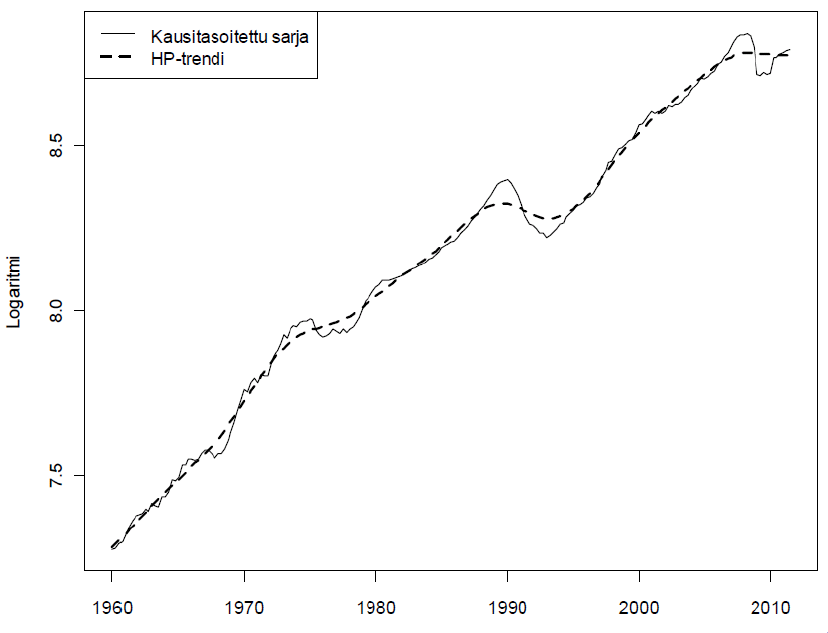
\includegraphics[width=0.6\textwidth]{./figures/aula14_fig1.PNG}
        \caption{PIB finlandês, $y_t$ e componente HP de tendência $g_t$. Fonte: Ahola (2012).}
        \label{fig1}
    \end{figure}
\end{frame}

\begin{frame}{Ciclos $\times$ passeios aleatórios}
    \begin{figure}
        \centering
        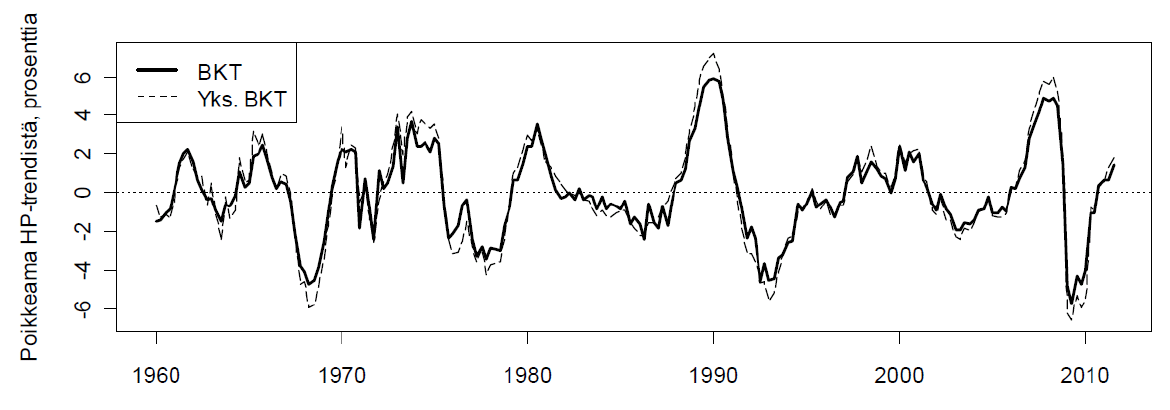
\includegraphics[width=\textwidth]{./figures/aula14_fig2.PNG}
        \caption{PIB finlandês, $y_t$ e componente HP cíclico $c_t = y_t - g_t$. Fonte: Ahola (2012).}
        \label{fig2}
    \end{figure}
\end{frame}

\begin{frame}{Ciclos $\times$ passeios aleatórios}
    \begin{itemize}
        \item Problemas com filtro HP:
        \begin{enumerate}
            \item Passa muitas flutuações de curto prazo (usar filtro bandpass, e.g., filtro BK).
            \bigskip
            \item É um filtro de médias móveis: problemas de ponto inicial e ponto terminal (perda de observações).
            \bigskip
            \item Cada variável tem seu próprio componente de tendência - algumas teorias dizem que deveria haver um componente comum.
            \bigskip
            \item \textcolor{purple}{Ciclos e tendência são independentes}.
        \end{enumerate}
    \end{itemize}
\end{frame}

\begin{frame}{Ciclos $\times$ passeios aleatórios}
    \begin{itemize}
        \item Nelson e Plosser (1982): ``modelos macro que focam em distúrbios monetários como fonte de flutuações puramente transitórias podem nunca ter sucesso em explicar uma grande fração da variação do produto, e a variação estocástica devido a fatores reais é um elemento essencial a qualquer modelo de flutuações macroeconômicas''.
        \bigskip
        \item \textcolor{purple}{Se fatores reais são responsáveis por flutuações agregadas, então, ciclos de negócios não podem ser vistos como eventos temporários}.
        \bigskip
        \item Recessões podem ter efeitos permanentes sobre o PIB.
    \end{itemize}
\end{frame}

\begin{frame}{Ciclos $\times$ passeios aleatórios}
    \begin{itemize}
        \item Procedimento econométrico:
        \[
        Y_t = g_t + bY_{t-1} + z_t.
        \]
        \bigskip
        \item Assume-se que o choque tem duração de um período.
        \bigskip
        \item Como $Y_t$ depende de $Y_{t-1}$, o choque se propagará ao longo do tempo, gerando correlação serial.
        \bigskip
        \item Se $0 < b < 1$ (abordagem convencional) o impacto do choque sobre o produto irá eventualmente desaparecer e o produto retorna à tendência de crescimento.
        \bigskip
        \item Neste caso, o produto é `estacionário em tendência' - Figura \ref{fig3}.
    \end{itemize}
\end{frame}

\begin{frame}{Ciclos $\times$ passeios aleatórios}
    \begin{figure}
        \centering
        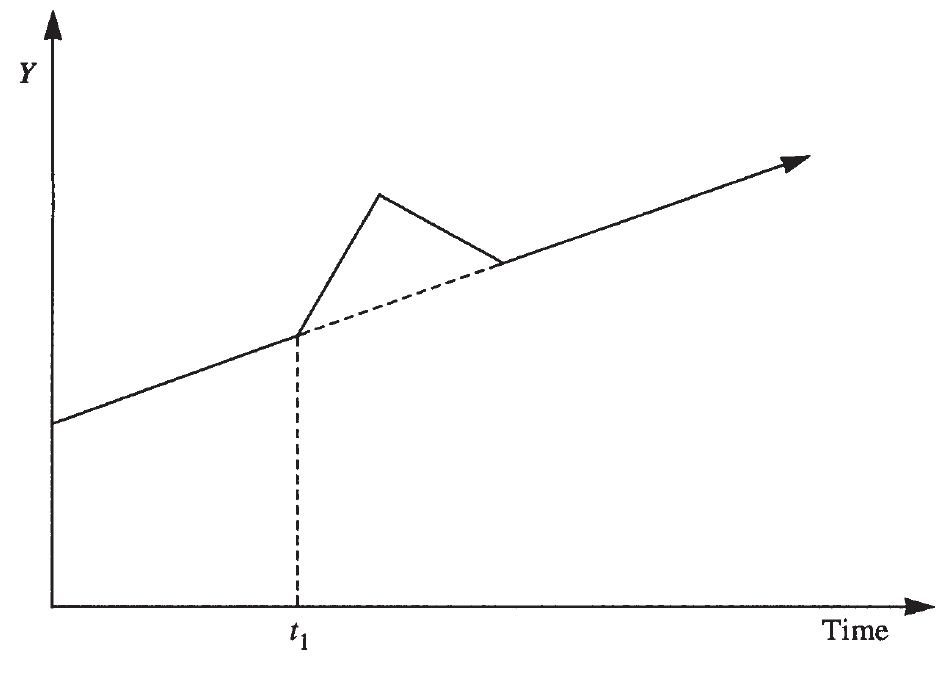
\includegraphics[width=0.6\textwidth]{./figures/aula14_fig3.PNG}
        \caption{Trajetória do produto no caso de estacionariedade em tendência. Fonte: Snowdon e Vane (2005).}
        \label{fig3}
    \end{figure}
\end{frame}

\begin{frame}{Ciclos $\times$ passeios aleatórios}
    \begin{itemize}
        \item Em contraste, Nelson e Plosser argumentam que a maior parte das variações que observamos é permanente, i.e., não há tendência de reversão à tendência após o choque.
        \bigskip
        \item Neste caso, o PIB evolui de acordo com um processo estatístico conhecido como \textcolor{purple}{passeio aleatório}.
        \bigskip
        \item Um passeio aleatório com deslocamento (drift) é dado por:
        \[
        Y_t = g_t + Y_{t-1} + z_t.
        \]
        \bigskip
        \item Neste caso, um choque positivo em $z$ irá aumentar o produto de forma permanente.
        \bigskip
        \item Diz-se que o produto possui uma raiz unitária.
        \bigskip
        \item Assume-se que a identificação de raízes unitárias é uma manifestação de choques à função de produção.
    \end{itemize}
\end{frame}

\begin{frame}{Ciclos $\times$ passeios aleatórios}
    \begin{figure}
        \centering
        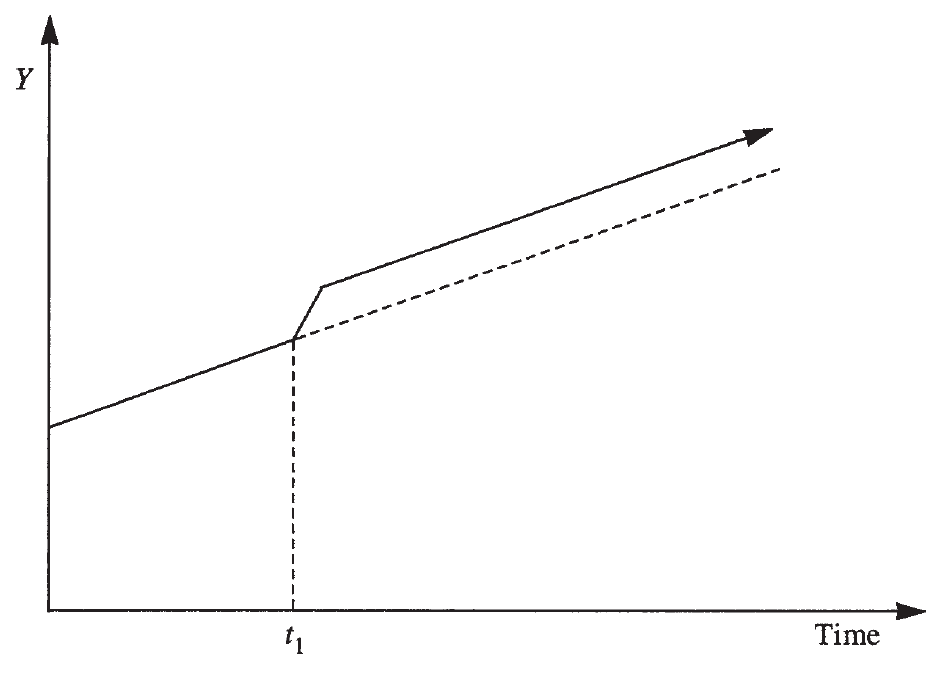
\includegraphics[width=0.6\textwidth]{./figures/aula14_fig4.PNG}
        \caption{Trajetória do produto no caso de choques com efeitos permanentes. Fonte: Snowdon e Vane (2005).}
        \label{fig4}
    \end{figure}
\end{frame}

\begin{frame}{Ciclos $\times$ passeios aleatórios}
    \begin{itemize}
        \item Se choques ao crescimento de produtividade devido a mudanças tecnológicas são frequentes e aleatórios, então, a trajetória do produto agregado seguindo um passeio aleatório irá exibir características similares a um ciclo econômico.
        \bigskip
        \item Neste caso, no entanto, as flutuações observadas são flutuações na taxa natural (tendência) do produto, e não desvios do produto com relação a um componente de tendência determinístico.
        \bigskip
        \item Segundo Nelson e Plosser, o que parece ser PIB flutuando ao redor de um componente de tendência suave é, na verdade, flutuação na taxa natural de produto induzida por uma série de choques permanentes, com cada novo choque permanente de produtividade determinando uma nova trajetória de crescimento.
    \end{itemize}
\end{frame}

\begin{frame}{Ciclos $\times$ passeios aleatórios}
    \begin{itemize}
        \item Seguindo o trabalho seminal de Solow, economistas tradicionalmente separaram a análise de crescimento econômico da análise de flutuações.
        \bigskip
        \item Nelson e Plosser sugerem que as forças econômicas determinantes do componente de tendência não são diferentes daquelas que causam flutuações.
        \bigskip
        \item Como mudanças permanentes no PIB não podem ser resultados de choques monetários (neutralidade da moeda), as principais forças causadoras de instabilidade devem ser choques reais.
        \bigskip
        \item Teorias monetárias tem importância limitada e distúrbios reais tendem a ser uma fonte muito mais significativa de instabilidade agregada.
        \bigskip
        \item Se há interações importantes entre os processos de crescimento e de ciclos de negócios, separar teoria do crescimento da análise de flutuações não é legítimo.
    \end{itemize}
\end{frame}

\subsection{Choques de oferta}
\begin{frame}{Choques de oferta}
    \begin{itemize}
        \item Instabilidade cíclica pode emergir por choques à demanda agregada ou de choques à oferta agregada, ou uma combinação dos dois.
        \bigskip
        \item Lado da demanda: choques podem originar de instabilidade de algum componente da curva IS (Keynes e modelos Keynesianos iniciais).
        \bigskip
        \item Lado da demanda: choques podem originar de instabilidade no lado monetário - curva IS e monetaristas.
    \end{itemize}
\end{frame}

\begin{frame}{Choques de oferta}
    \begin{itemize}
        \item Lado da oferta: temos uma variedade de choques que podem resultar em variações significativas na produtividade.
        \bigskip
        \begin{enumerate}
            \item Desenvolvimentos negativos no ambiente físico que afetam de maneira adversa o produto agrícola, e.g., desastres naturais como terremotos, secas e inundações.
            \bigskip
            \item Choques nos preços de energia, e.g., choques do petróleo. Hamilton (1983, 1996) argumenta que a maioria das recessões EUA desde 1945 foram precedidas por aumentos nos preços de energia.
            \bigskip
            \item Guerras, agitações políticas ou trabalhistas que perturbam a performance e estrutura da economia, e.g., Iugoslávia, União Soviética, Iraque, ou greves trabalhistas no UK durante 1970s e 1984.
            \bigskip
            \item Regulações governamentais como quotas de importação - distorcem incentivos e deslocam empreendedorismo em direção a atividades rentistas.
            \bigskip
            \item \textcolor{purple}{Choques de produtividade gerados por mudanças na qualidade dos insumos capital e trabalho, novas práticas de gerenciamento, desenvolvimento de novos produtos e introdução de novas técnicas de produção}.
        \end{enumerate}
    \end{itemize}
\end{frame}

\subsection{Ciclos de negócios: fatos estilizados}
\begin{frame}{Ciclos de negócios: fatos estilizados}
    \begin{itemize}
        \item \textcolor{blue}{Fatos estilizados}: regularidades identificadas nas propriedades estatísticas das séries temporais econômicas.
        \bigskip
        \item Explicações teóricas do fenômeno de ciclos de negócios devem ser guiadas pelas propriedades estatísticas identificadas dos comovimentos dos desvios com relação à tendência de vários agregados econômicos com relação ao PIB real.
        \bigskip
        \item A capacidade de uma teoria em particular de replicar os principais fatos estilizados será um fator determinante de avaliação desta teoria:
        \begin{quote}
            Para obter sucesso, uma teoria do ciclo de negócio deve explicar o comportamento cíclico não apenas de algumas poucas variáveis, como produto e emprego, mas de um grande número de variáveis econômicas chaves.
        \end{quote}
        \begin{flushright}
            Abel e Bernanke (2001).
        \end{flushright}
    \end{itemize}
\end{frame}

\begin{frame}{Ciclos de negócios: fatos estilizados}
    \begin{figure}
        \centering
        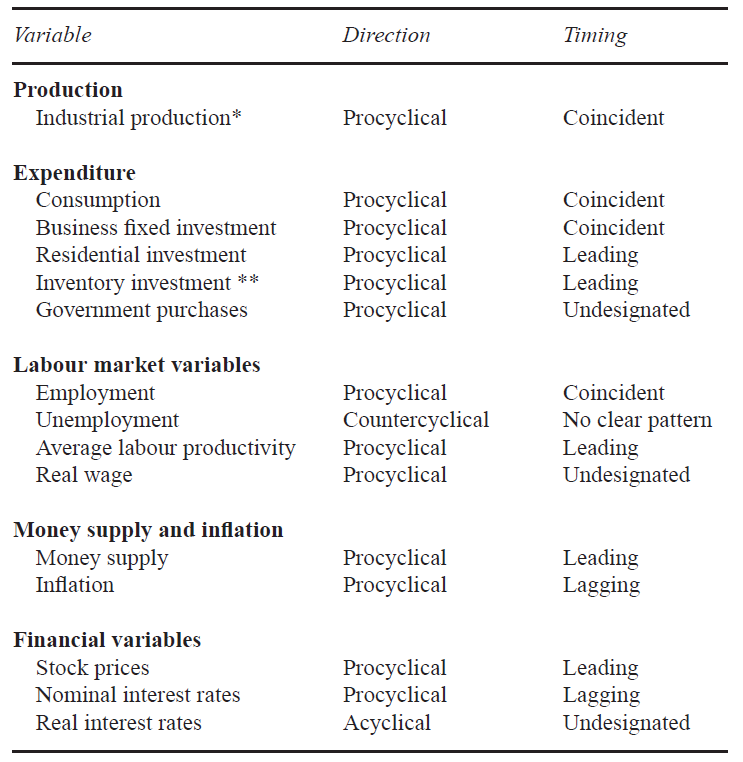
\includegraphics[width=0.4\textwidth]{./figures/aula14_fig5.PNG}
        \caption{Fatos estilizados do ciclo de negócios. Fonte: Snowdon e Vane (2005).}
        \label{fig5}
    \end{figure}
\end{frame}

\section{Modelo de Ciclos Reais de Negócios (RBC)}
\subsection{Introdução}
\begin{frame}{Modelo RBC: Introdução}
    \begin{itemize}
        \item Kydland e Prescott iniciaram o programa de pesquisa RBC com a
ideia de que crescimento e ciclos não são fenômenos distintos e
seguiram o desafio de Lucas de criar uma economia artificial que
conseguisse imitar a economia real.
\bigskip
\item A economia artificial contém agentes otimizadores interagindo em um
ambiente competitivo sem fricções que é sujeito a choques de
produtividade.
\bigskip
\item Essa nova fase de modelos novo-clássicos enfatiza choques reais de tecnologia como impulso dos ciclos econômicos em detrimento a
choques monetários.
    \end{itemize}
\end{frame}

\begin{frame}{Modelo RBC: Introdução}
    \begin{itemize}
        \item Seguindo Frisch (1933) e Lucas (1977), modelos RBC distinguem mecanismos de \textcolor{purple}{impulso} e de \textcolor{purple}{propagação} e têm as seguintes características:
        \bigskip
        \begin{enumerate}
            \item Agentes que maximizam funções objetivo sujeitas a restrições.
            \bigskip
            \item Expectativas racionais e ausência de assimetria de informações.
            \bigskip
            \item Equilíbrio contínuo sem custos de transação ou fricções.
            \bigskip
            \item Choques tecnológicos exógenos são o mecanismo de impulso.
            \bigskip
            \item Suavização de C, substituição entre L e N propagam os impulsos.
            \bigskip
            \item Flutuações no emprego são voluntárias.
            \bigskip
            \item Política monetária é irrelevante e moeda é neutra.
            \bigskip
            \item Distinção entre curto e longo prazo abandonada.
        \end{enumerate}
    \end{itemize}
\end{frame}

\subsection{Estrutura teórica}
\begin{frame}{Modelo RBC: Estrutura teórica}
    \begin{itemize}
        \item A produção agregada do bem único, usado tanto para C quanto para I, é
feita por uma função de produção com retornos constantes de escala:
\begin{equation}
    Y_t = Z_t F(K_t, N_t),
    \label{eq1}
\end{equation}
com $\log(Z_{t}) = (1-\rho)\log(\bar{Z}) + \rho \log(Z_{t-1}) + \varepsilon_t, \qquad \varepsilon_t \sim i.i.d. \mathcal{N}(0, \sigma^2)$.
\bigskip
\item A função utilidade do consumidor representativo deve satisfazer:
\begin{equation*}
    U(C_t, N_t), \qquad U_C(C_t, N_t) > 0, \quad U_N(C_t, N_t) < 0.
\end{equation*}
\bigskip
    \item O objetivo do consumidor representativo é maximizar o VPL das utilidades presente e futuras em um horizonte infinito, sujeito às restrições da economia:
    \begin{eqnarray*}
    Y_t &=& C_t + I_t, \\
    K_{t+1} &=& I_t + (1-\delta)K_t.
    \end{eqnarray*}
    \end{itemize}
\end{frame}

\begin{frame}{Modelo RBC: Problema de otimização}
    \begin{equation}
        \max_{C_t, N_t} \mathbb{E}_t\left[\sum_{j=0}^\infty \beta^{t+j} \left(\left. \frac{C_{t+j}^{1-\phi}-1}{1-\phi} - AN_{t+j}\right) \right| \Omega_t \right]
        \label{eq2}
    \end{equation}
    sujeito às restrições:
    \begin{eqnarray}
    C_t + I_t &=& Z_tF(K_t, N_t) = Y_t, \nonumber \\
    K_{t+1} &=& I_t + (1-\delta)K_t, \label{eq3} \\
    \log(Z_t) &=& (1-\rho)\log(\bar{Z}) + \rho \log (Z_{t-1}) + \varepsilon_t. \nonumber
    \end{eqnarray}
    \bigskip
    \begin{itemize}
        \item Seria possível modelar crescimento econômico através de progresso tecnológico neutro de Harrod em $N_t$.
        \bigskip
        \item O ciclo econômico será gerado pelos diferentes incentivos a trabalho e
lazer no presente e no futuro dados por choques tecnológicos
positivos e negativos.
    \end{itemize}
\end{frame}

\begin{frame}{Lagrangeano}
    [Na lousa.]
\end{frame}

\begin{frame}{Condição Intratemporal}
    \begin{itemize}
        \item Como temos mercados perfeitamente competitivos, o retorno bruto do capital é dado por:
        \[
        R_t = 1 - \delta + Z_tF_K(K_t, N_t).
        \]
        \bigskip
        \item O salário real é dado pela produtividade marginal do trabalho:
        \[
        W_t = Z_t F_N(K_t, N_t).
        \]
        \bigskip
        \item As CPOs podem ser reescritas como:
        \begin{eqnarray}
            C_t^{-\phi} &=& \lambda_t, \label{eq4} \\
            A &=& \lambda_t W_t, \label{eq5} \\
            \lambda_t &=& \beta \mathbb{E}[\lambda_{t+1}R_{t+1}|\Omega_t]. \label{eq6}
        \end{eqnarray}
    \end{itemize}
\end{frame}

\begin{frame}{Condição Intratemporal}
    \begin{itemize}
        \item Combinando as equações (\ref{eq4}) e (\ref{eq5}), obtemos a \textcolor{purple}{condição intratemporal}:
        \begin{equation}
            A = C_t^{-\phi}W_t = C_t^{-\phi}Z_t F_N(K_t, N_t). \label{eq7}
        \end{equation}
        \bigskip
        \item A equação (\ref{eq7}) diz que $-U_N$ deve ser igual a $U_C$ vezes o salário real, mostrando como choques em $Z_t$ geram variações em $W_t$ e, consequentemente, na oferta de trabalho.
    \end{itemize}
\end{frame}

\begin{frame}{Condição Intertemporal}
    \begin{itemize}
        \item A equação de Euler ou \textcolor{purple}{condição intertemporal} é dada por:
        \begin{equation}
            C_t^{-\phi} = \beta \mathbb{E}[C_{t+1}^{-\phi} R_{t+1}|\Omega_t]. \label{eq8}
        \end{equation}
        \bigskip
        \item A equação (\ref{eq8}) regula a condição de suavização e/ou oscilação do consumo.
        \bigskip
        \item A abdicação de $-\Delta C_t$ hoje gera $-\Delta C_t \times C_t^{-\phi}$ de perda em $U$, mas $\Delta C_t$ pode ser alocado em capital e ser remunerado à taxa $R_{t+1}$.
        \bigskip
        \item Note que este investimento gerará $\mathbb{E}[C_{t+1}^{-\phi} R_{t+1}|\Omega_t]$ em $t+1$.
        \bigskip
        \item A equação (\ref{eq8}) diz que em uma trajetória ótima, o consumidor deve ser indiferente a estas opções.
    \end{itemize}
\end{frame}

\begin{frame}{Condição Intertemporal}
    \begin{itemize}
        \item Rearranjando a equação (\ref{eq8}) e ignorando, por hora, a incerteza, temos:
        \[
        \frac{C_{t+1}}{C_t} = (\beta R_{t+1})^{1/\phi}.
        \]
        \bigskip
        \item Se $\beta R_{t+1} = 1$, então $\frac{C_{t+1}}{C_t} = 1$ e o consumo será suavizado ao longo da vida.
        \bigskip
        \item Se $\beta R_{t+1} \neq 1$, também haverá tendência a suavização se $\phi \to \infty$, pois $\frac{C_{t+1}}{C_t} \to 1$.
        \bigskip
        \item Se $\phi \to 0$, então $\frac{C_{t+1}}{C_t} \to \infty$ e haverá tendência a explorar diferenças entre $\beta$ e $R_{t+1}$.
    \end{itemize}
\end{frame}

\subsection{Mecanismos de propagação de choques}
\begin{frame}{Efeito de choques tecnológicos: Consumo intertemporal}
    \begin{itemize}
        \item Suponha que um choque tecnológico positivo afeta a economia, ou seja, $+\Delta Z_t$, logo $Y_t = Z_tF(K_t,N_t) \uparrow$.
        \bigskip
        \item Como $\uparrow R_t$, haverá incentivo a poupar mais hoje para consumir mais no futuro (\textcolor{purple}{efeito substituição}), mas este incentivo dependerá da duração do choque.
        \bigskip
        \item Além disso, $W_t = Z_t F_N(K_t,N_t) \uparrow$ e o consumidor tenderá a consumir mais hoje devido à renda maior (\textcolor{blue}{efeito renda}).
        \bigskip
        \item Se o choque for permanente, $\Delta C_t = \Delta Y_t, \quad \forall t$ e o efeito renda dominará totalmente.
        \bigskip
        \item Mas se o choque for temporário, o consumidor irá explorar $\uparrow R$ para investir agora e consumir mais no futuro, fazendo com que $\Delta Y_t = \Delta C_t + \Delta I_t$.
    \end{itemize}
\end{frame}

\begin{frame}{Efeito de choques tecnológicos: Consumo intertemporal}
    \begin{itemize}
        \item Quanto maior (menor) for a persistência de $Z_t$, maior (menor) será o efeito renda.
        \bigskip
        \item Como nas observações empíricas $C_t$ flutua proporcionalmente menos do que $Y_t$ - Figura \ref{fig6}, os choques tecnológicos são calibrados de forma a serem muito persistentes (efeito renda forte), porém não permanentes, permitindo algum efeito substituição.
    \end{itemize}
\end{frame}

\begin{frame}{Efeito de choques tecnológicos: Consumo intertemporal}
    \begin{figure}
        \centering
        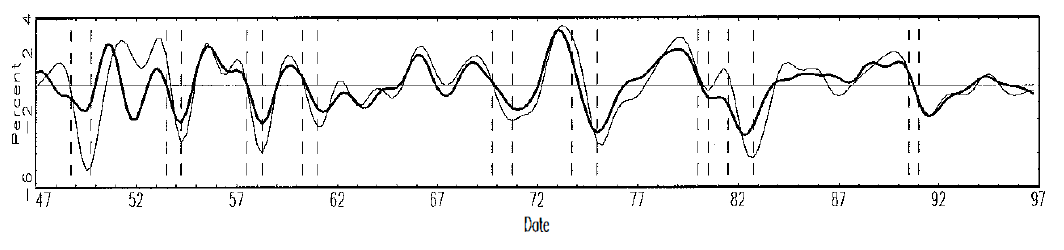
\includegraphics[width=1\textwidth]{./figures/aula14_fig6.PNG}
        \caption{Componente cíclico: Consumo total (linha grossa) e PIB (linha fina). Fonte: Stock e Watson (1999).}
        \label{fig6}
    \end{figure}
\end{frame}

\begin{frame}{Efeito de choques tecnológicos: Decisão trabalho e lazer}
    \begin{itemize}
        \item Se $\uparrow Z_t$, então $\uparrow W_t$ incentivará também a substituição intertemporal de $N_t$.
        \bigskip
        \item Porém, $\uparrow W_t$ faz com que o consumidor se sinta mais rico (efeito renda) e queira consumir mais lazer, forçando $\downarrow N_t$.
        \bigskip
        \item Se $+\Delta Z_t$ for permanente, o efeito renda dominará, mas para choques temporários a resposta de $N_t$ é ambígua.
        \bigskip
        \item Caso $+\Delta Z_t$ for transitório e $\uparrow N_t$, o trabalho adicional gerará investimento e, com isso, o consumo futuro será maior mesmo após o fim do choque.
        \bigskip
        \item Nos dados, pequenas alterações em $W_t$ geram grandes variações em $N_t$. Para ajustar o modelo a essa evidência, o efeito substituição precisa ser alto.
        \bigskip
        \item Note que essas flutuações em $Y, C, I$ e $N$ são ótimas do ponto de vista do consumidor e não há motivos para intervenção do governo.
    \end{itemize}
\end{frame}

\begin{frame}{Choque tecnológico e oferta de trabalho}
    \begin{figure}
        \centering
        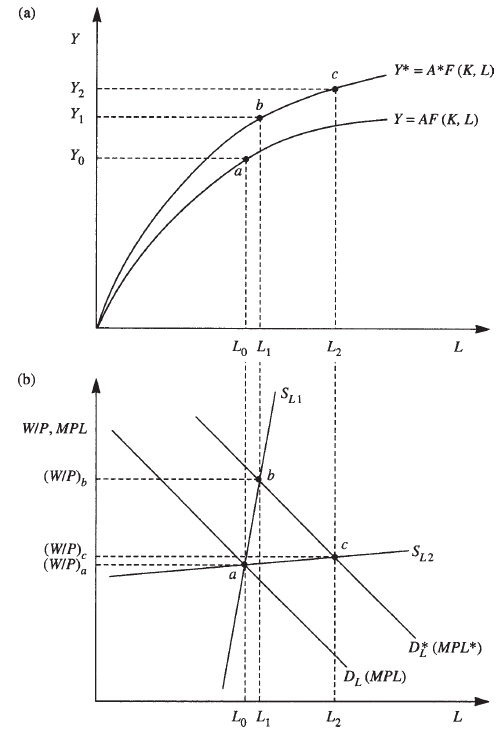
\includegraphics[width=0.3\textwidth]{./figures/aula14_fig7.PNG}
        \caption{Choque tecnológico: flutuações no emprego e produto. Fonte: Snowdon e Vane (2005).}
        \label{fig7}
    \end{figure}
\end{frame}

\begin{frame}{Decisão entre trabalho e lazer: lado do consumo}
    \begin{itemize}
        \item As equações (\ref{eq7})-(\ref{eq8}) representam as decisões ótimas de famílias e firmas, mas não permitem encontrar as funções política analíticas $C_t(K_t, Z_t)$ e $N_t(K_t, Z_t)$.
        \medskip
        \item Para facilitar a solução analítica, faremos $\phi = 1$.
        \medskip
        \item Quando $\phi \to 1$, $U(C) \to \ln C$ pois pela regra de L'Hospital:
        \begin{eqnarray*}
        \lim_{\phi \to 1} \frac{C^{1-\phi}-1}{1-\phi} &=& \lim_{\phi \to 1} \frac{(C^{1-\phi} \ln C) (-1)}{-1} = \lim_{\phi \to 1} C^{1-\phi}\ln C \\
        &=& \ln C \lim_{\phi \to 1} C^{1-\phi} = \ln C.
        \end{eqnarray*}
        \medskip
        \item Podemos representar a decisão das famílias entre consumo e trabalho usando curvas de indiferença.
        \medskip
        \item As curvas de indiferença terão inclinação negativa no plano consumo e lazer, e positiva no plano consumo e trabalho.
        \medskip
        \item A TMS entre consumo e lazer nos diz o quanto a mais de consumo será necessário para compensar uma perda de horas de lazer.
    \end{itemize}
\end{frame}

\begin{frame}{Função utilidade e curvas de indiferença}
    \begin{figure}
        \centering
        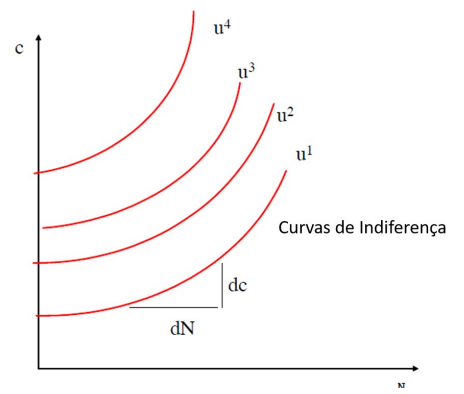
\includegraphics[width=0.5\textwidth]{./figures/aula14_fig8.PNG}
        \caption{Função utilidade e curvas de indiferença. Fonte: Moura (2017).}
        \label{fig8}
    \end{figure}
\end{frame}

\begin{frame}{Decisão entre trabalho e lazer: lado da produção}
    \begin{itemize}
        \item Para possibilitar a solução analítica, retiraremos o estoque de capital da função de produção e faremos:
        \[
        F = ZN^{1-\alpha}.
        \]
        \bigskip
        \item Com isso, a produtividade marginal do trabalho será dada por:
        \begin{eqnarray*}
        F_N &=& (1-\alpha)ZN^{-\alpha} > 0, \\
        F_{N^2} &=& \alpha(\alpha-1)ZN^{-\alpha-1} < 0.
        \end{eqnarray*}
        \bigskip
        \item Note que como não há estoque de capital, não há decisão intertemporal, a restrição da economia que era $Y = C + I$ se torna simplesmente $Y = C$ e a análise é estática.
    \end{itemize}
\end{frame}

\begin{frame}{Decisão entre trabalho e lazer: lado da produção}
    \begin{figure}
        \centering
        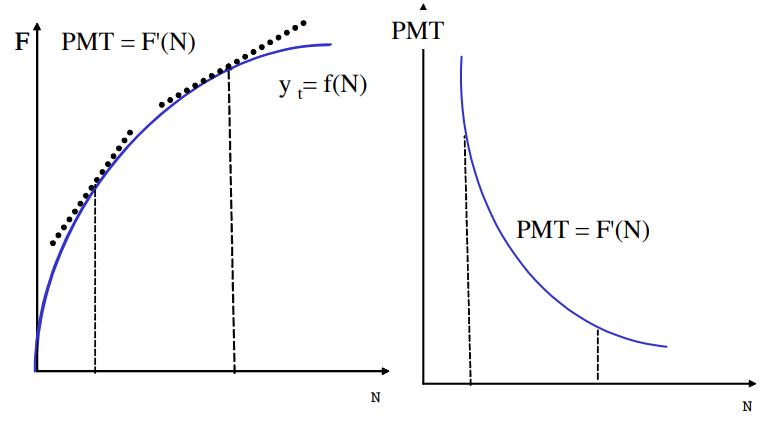
\includegraphics[width=0.8\textwidth]{./figures/aula14_fig9.PNG}
        \caption{Produtividade marginal do trabalho. Fonte: Moura (2017).}
        \label{fig9}
    \end{figure}
\end{frame}

\begin{frame}{Equilíbrio geral: representação gráfica}
    \begin{figure}
        \centering
        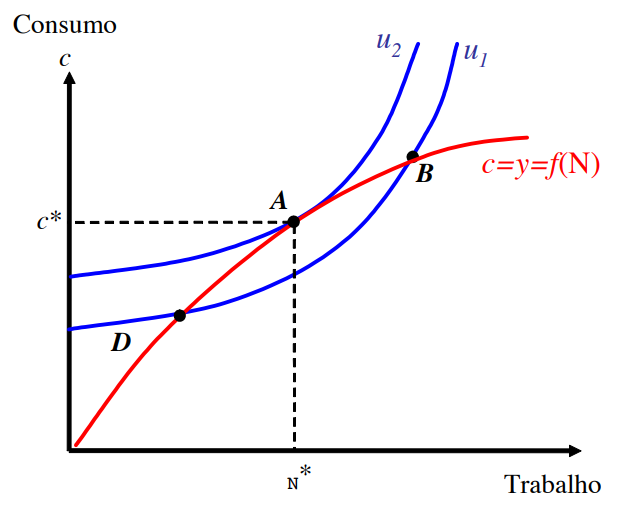
\includegraphics[width=0.5\textwidth]{./figures/aula14_fig10.PNG}
        \caption{Equilíbrio geral: consumo $\times$ produção. Fonte: Moura (2017).}
        \label{fig10}
    \end{figure}
\end{frame}

\begin{frame}{Equilíbrio geral: Consumo e produção}
    \begin{itemize}
        \item A CPO do problema:
        \begin{equation}
            \max_{C, (1-N)} \ln (C) - AN, \qquad \text{s.r.} \quad C = ZN^{1-\alpha}. \label{eq9}
        \end{equation}
        é dada por:
        \begin{eqnarray*}
        TMS = AC = AY &\doteq& (1-\alpha)ZN^{-\alpha} = (1-\alpha)\frac{Y}{N} = PMg_N \\
        &\Rightarrow& N(\bullet) = \frac{1-\alpha}{A}.
        \end{eqnarray*}
        \bigskip
        \item Portanto, a função política para o consumo é dada por:
        \[
        C(Z) = Y = ZN^{1-\alpha} = Z\left(\frac{1-\alpha}{A} \right)^{1-\alpha}.
        \]
    \end{itemize}
\end{frame}

\begin{frame}{Equilíbrio geral: consumo e produção}
    \begin{itemize}
        \item Segue que:
        \begin{eqnarray*}
        \frac{\partial N(Z)}{\partial (1-\alpha)} &>& 0, \\
        \frac{\partial N(Z)}{\partial Z} &=& 0, \\
        \frac{\partial N(Z)}{\partial A} &<& 0.
        \end{eqnarray*}
        \bigskip
        \item Enquanto:
        \begin{eqnarray*}
        \frac{\partial C(Z)}{\partial (1-\alpha)} &>& 0, \\
        \frac{\partial C(Z)}{\partial Z} &>& 0, \\
        \frac{\partial C(Z)}{\partial A} &<& 0.
        \end{eqnarray*}
    \end{itemize}
\end{frame}

\begin{frame}{Deslocamento paralelo na função de produção}
    \begin{figure}
        \centering
        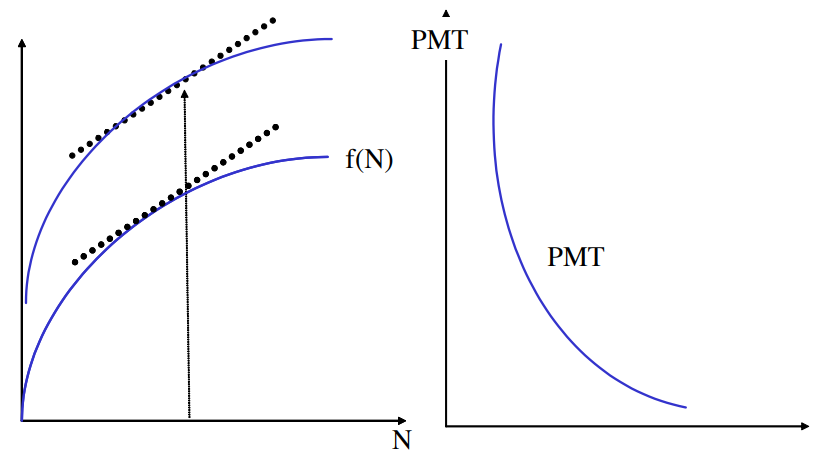
\includegraphics[width=0.8\textwidth]{./figures/aula14_fig11.PNG}
        \caption{Deslocamento paralelo na função de produção. Fonte: Moura (2017).}
        \label{fig11}
    \end{figure}
\end{frame}

\begin{frame}{Choque tecnológico positivo (choque na PTF)}
    \begin{figure}
        \centering
        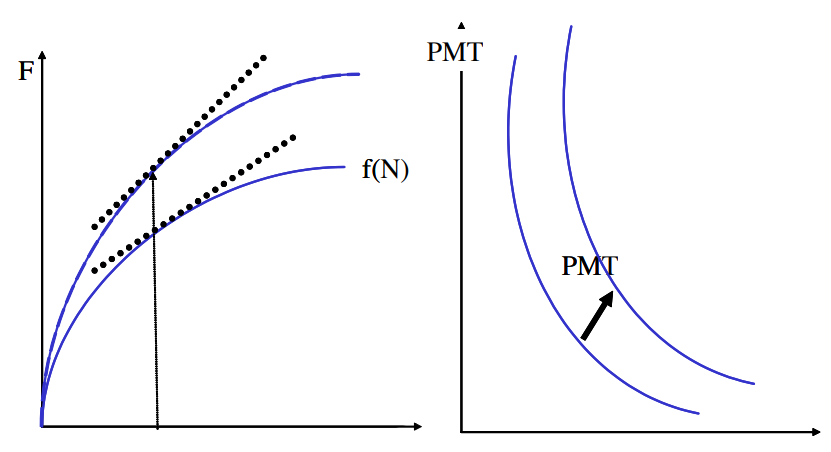
\includegraphics[width=0.8\textwidth]{./figures/aula14_fig12.PNG}
        \caption{Choque tecnológico positivo e $PMg_N$. Fonte: Moura (2017).}
        \label{fig12}
    \end{figure}
\end{frame}

\begin{frame}{Efeitos renda e substituição}
    \begin{itemize}
        \item \textcolor{purple}{Efeito renda}: um aumento da renda para qualquer escolha de $N$, porém mantendo a relação do $PMg_N$ inalterada.
        \bigskip
        \item \textcolor{blue}{Efeito substituição}: mudança somente na relação do $PMg_N$, mas não na renda em si.
        \bigskip
        \item Um aumento em $Z$ gerará tanto efeito renda como substituição.
        \bigskip
        \item As formas das funções utilidade e de produção irão determinar qual efeito será maior.
        \bigskip
        \item Usando a função utilidade separável e logarítmica, bem como a função exponencial anterior, vimos que estes efeitos se cancelam e o consumidor não altera a oferta de trabalho.
    \end{itemize}
\end{frame}

\begin{frame}{Choque PTF: efeitos renda e substituição}
    \begin{itemize}
        \item Supondo ainda que o consumidor obtenha renda exógena $X$ e que $F$ seja linear $(1-\alpha = 1)$, é possível observar o efeito total positivo na oferta de trabalho.
    \end{itemize}
    \begin{figure}
        \centering
        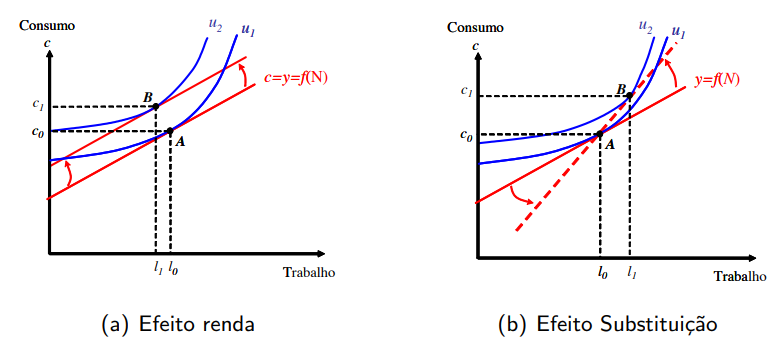
\includegraphics[width=0.7\textwidth]{./figures/aula14_fig13.PNG}
        \caption{Efeitos renda e substituição. Fonte: Moura (2017).}
        \label{fig13}
    \end{figure}
\end{frame}

\begin{frame}{Equação de Slutsky}
    \begin{figure}
        \centering
        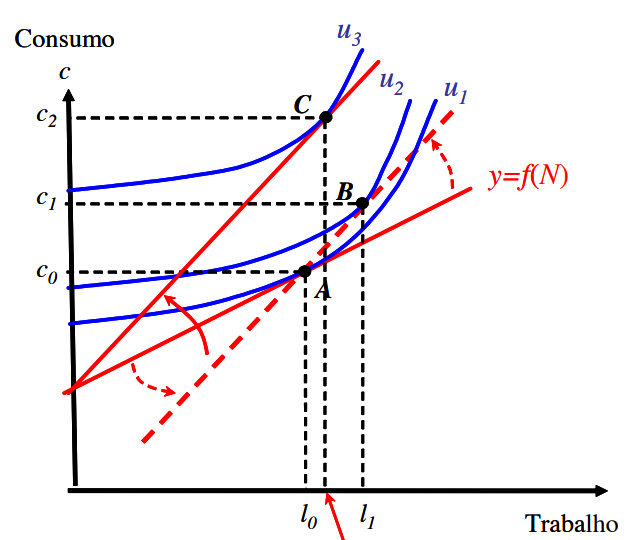
\includegraphics[width=0.5\textwidth]{./figures/aula14_fig14.PNG}
        \caption{Efeito total - equação de Slutsky. Fonte: Moura (2017).}
        \label{fig14}
    \end{figure}
\end{frame}

\begin{frame}{Solução do modelo completo}
    \begin{itemize}
        \item Para entendermos os efeitos dos choques no modelo completo, precisamos resolver as CPOs para encontrarmos as funções políticas $C(K_t, Z_t)$ e $N(K_t, Z_t)$.
        \bigskip
        \item Entretanto, as equações (\ref{eq7})-(\ref{eq8}) formam um sistema de equações não-lineares sem solução analítica.
        \bigskip
        \item A estratégia usual para encontrar as funções políticas é a log-linearização do sistema de CPOs ao redor do estado estacionário para obtermos um sistema linear, facilitando também a solução da esperança em (\ref{eq8}).
        \bigskip
        \item Após a log-linearização, é possível utilizar o procedimento desenvolvido por Blanchard e Kahn (1980) ou o método de coeficientes a determinar para solucionar sistemas lineares de expectativas racionais.
        \bigskip
        \item Para mais detalhes, ver Uhlig (2000) e/ou DeJong e Dave (2011).
    \end{itemize}
\end{frame}

\section{Bibliografia}
\begin{frame}{\emoji{books} Bibliografia}
    \begin{itemize}                        
        \item Alesina, A. and Roubini, N. with Cohen, G.D. (1997), Political Cycles and the Macroeconomy: Theory and Evidence, Cambridge, MA: MIT Press\medskip
        \item Alesina, A. and Summers, L.H. (1993), ‘Central Bank Independence and Macroeconomic Performance: Some Comparative Evidence’, Journal of Money, Credit, and Banking\medskip
        \item Barro, R.J. (1977), ‘Unanticipated Money Growth and Unemployment in the United States’, American Economic Review\medskip
        \item Barro, R.J. (1978), ‘Unanticipated Money, Output and the Price Level in the United States’, Journal of Political Economy\medskip
        \item Barro, R.J. and Gordon, D.B. (1983), ‘Rules, Discretion and Reputation in a Model of Monetary Policy’, Journal of Monetary Economics\medskip
        \item Blackburn, K. (1992), ‘Credibility and Time-Consistency in Monetary Policy’, in K. Dowd and M.K. Lewis (eds), Current Issues in Financial and Monetary Economics, Basingstoke: Macmillan\medskip
        \item Blanchard, O.J. (1984), ‘The Lucas Critique and the Volcker Deflation’, American Economic Review\medskip
        \item Buiter, W.H. (1980), ‘The Macroeconomics of Dr. Pangloss: A Critical Survey of the New Classical Macroeconomics’, Economic Journal\medskip        
    \end{itemize}
\end{frame}

\begin{frame}{\emoji{books} Bibliografia}
    \begin{itemize}                        
        \item Cross, R. (ed.) (1988), Unemployment, Hysteresis and the Natural Rate Hypothesis, Oxford: Basil Blackwell\medskip        
        \item Drazen, A. (2000a), Political Economy in Macroeconomics, Princeton: Princeton University Press\medskip
        \item Fischer, S. (1977), ‘Long-Term Contracts, Rational Expectations, and the Optimal Money Supply Rule’, Journal of Political Economy\medskip
        \item Friedman, M. (1968), ‘The Role of Monetary Policy’, American Economic Review\medskip        
        \item Gordon, R.J. (1978), ‘What Can Stabilisation Policy Achieve?’, American Economic Review\medskip
        \item Gordon, R.J. (1982), ‘Price Inertia and Policy Ineffectiveness in the United States, 1890–1980’, Journal of Political Economy\medskip
        \item Gordon, R.J. (1988), ‘Hysteresis in History: Was There Ever a Phillips Curve?’, American Economic Review\medskip
        \item Hahn, F. (1982), Money and Inflation, Oxford: Basil Blackwell\medskip
        \item Hoover, K.D. (ed.) (1995), Macroeconometrics: Developments, Tensions and Prospects, Boston, MA: Kluwer Academic Publishers\medskip        
    \end{itemize}
\end{frame}

\begin{frame}{\emoji{books} Bibliografia}
    \begin{itemize}                        
        \item Koopmans, T.C. (1949), ‘The Econometric Approach to Business Fluctuations’, American Economic Review\medskip        
        \item Kydland, F.E. and Prescott, E.C. (1977), ‘Rules Rather Than Discretion: The Inconsistency of Optimal Plans’, Journal of Political Economy\medskip
        \item Lucas, R.E. Jr (1972), ‘Expectations and the Neutrality of Money’, Journal of Economic Theory\medskip
        \item Lucas, R.E. Jr (1975), ‘An Equilibrium Model of the Business Cycle’, Journal of Political Economy\medskip
        \item Lucas, R.E. Jr (1976), ‘Econometric Policy Evaluation: A Critique’, in K. Brunner and A. Meltzer (eds), The Phillips Curve and Labor Markets, Amsterdam: North-Holland, Carnegie-Rochester Series on Public Policy\medskip
        \item Lucas, R.E. Jr (1977), ‘Understanding Business Cycles’, in K. Brunner and A.H. Meltzer (eds), Stabilization of the Domestic and International Economy, Amsterdam and New York: North-Holland\medskip
        \item Lucas, R.E. Jr (2003), ‘Macroeconomic Priorities’, American Economic Review\medskip
        \item Lucas, R.E. Jr and Rapping, L.A. (1969), ‘Real Wages, Employment and Inflation’, Journal of Political Economy\medskip        
    \end{itemize}
\end{frame}

\begin{frame}{\emoji{books} Bibliografia}
    \begin{itemize}                        
        \item Mishkin, F.S (1982), ‘Does Anticipated Monetary Policy Matter? An Econometric Investigation’, Journal of Political Economy\medskip        
        \item Modigliani, F. (1996), ‘The Shameful Rate of Unemployment in the EMS: Causes and Cures’, De Economist\medskip
        \item Muth, J.F. (1961), ‘Rational Expectations and the Theory of Price Movements’,  Econometrica\medskip        
        \item Phelps, E.S. and Taylor, J.B. (1977), ‘Stabilizing Powers of Monetary Policy Under Rational Expectations’, Journal of Political Economy\medskip
        \item Rogoff, K. (1985), ‘The Optimal Degree of Commitment to an Intermediate Monetary Target’, Quarterly Journal of Economics\medskip
        \item Sargent, T.J. and Wallace, N. (1975), ‘Rational Expectations, the Optimal Monetary Instrument and the Optimal Money Supply Rule’, Journal of Political Economy\medskip
        \item Sargent, T.J. and Wallace, N. (1976), ‘Rational Expectations and the Theory of Economic Policy’, Journal of Monetary Economics\medskip
        \item SNOWDON, B.; VANE, H.R. \emph{Modern Macroeconomics: its Origins, Development and Current State}. Northampton, MA: Edward Elgar, 2005\medskip                
    \end{itemize}
\end{frame}

\begin{frame}{\emoji{books} Bibliografia}
    \begin{itemize}                        
        \item Solow, R.M. (1998), ‘How Cautious Must the Fed Be?’, in R.M. Solow and J.B. Taylor, Inflation, Unemployment and Monetary Policy, Cambridge, MA: MIT Press\medskip        
        \item Svensson, L.E.O. (1997), ‘Optimal Inflation Targets, “Conservative” Central Banks and Linear Inflation Contracts’, American Economic Review\medskip
        \item Taylor, H. (1985), ‘Time Inconsistency: A Potential Problem for Policymakers’, Federal Reserve Bank of Philadelphia Business Review\medskip
        \item Taylor, J.B. (1980), ‘Aggregate Dynamics and Staggered Contracts’, Journal of Political Economy\medskip
        \item Waller, C.J. and Walsh, C.E. (1996), ‘Central Bank Independence, Economic Behaviour and Optimal Term Lengths’, American Economic Review\medskip
        \item Walsh, C.E. (1993), ‘Central Bank Strategies, Credibility and Independence: A Review Essay’, Journal of Monetary Economics\medskip
        \item Walsh, C.E. (1995), ‘Optimal Contracts for Central Bankers’, American Economic Review\medskip
    \end{itemize}
\end{frame}
\end{document}